%第3章



\section{基本設計}

問題領域やシステムの構造を論理的,静的にみるためにクラス図を作成した.以下にICタグを用いた商品識別システムのクラス図として,図\ref{class_ic}を載せる.

\begin{figure}[htbp]
\centering
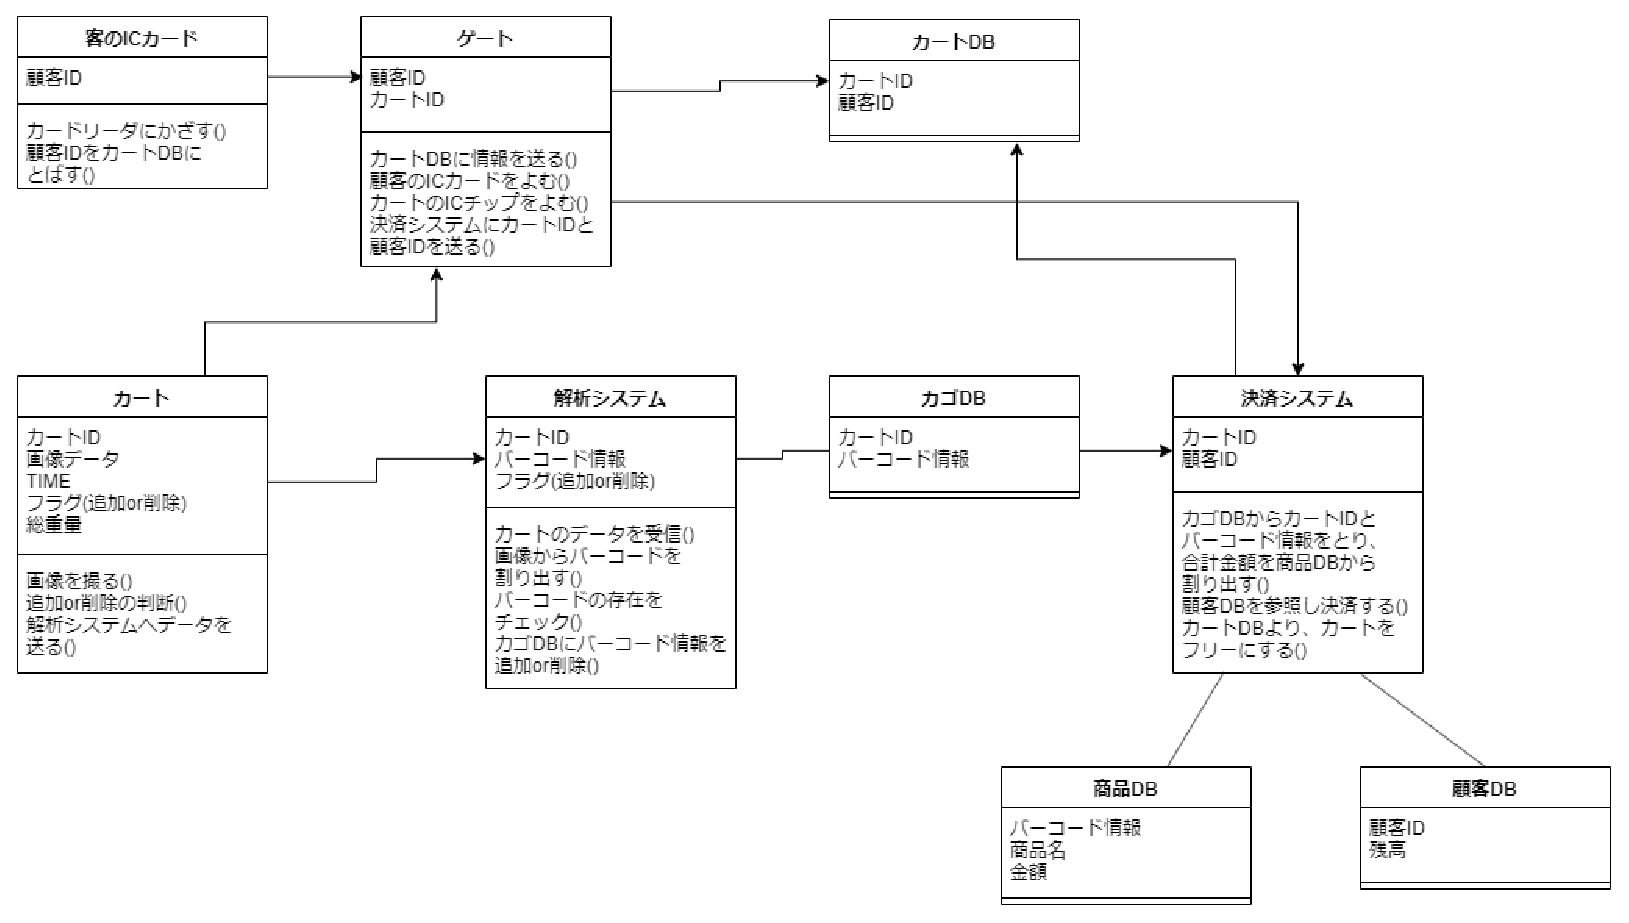
\includegraphics[width=15cm]{./picture/class_ic.eps}
\caption{ICタグを用いたシステムのクラス図}
\label{class_ic}
\end{figure}


以下にQRコードを用いた商品識別システムのクラス図,図\ref{class_qr}を載せる.


\begin{figure}[htbp]
\centering
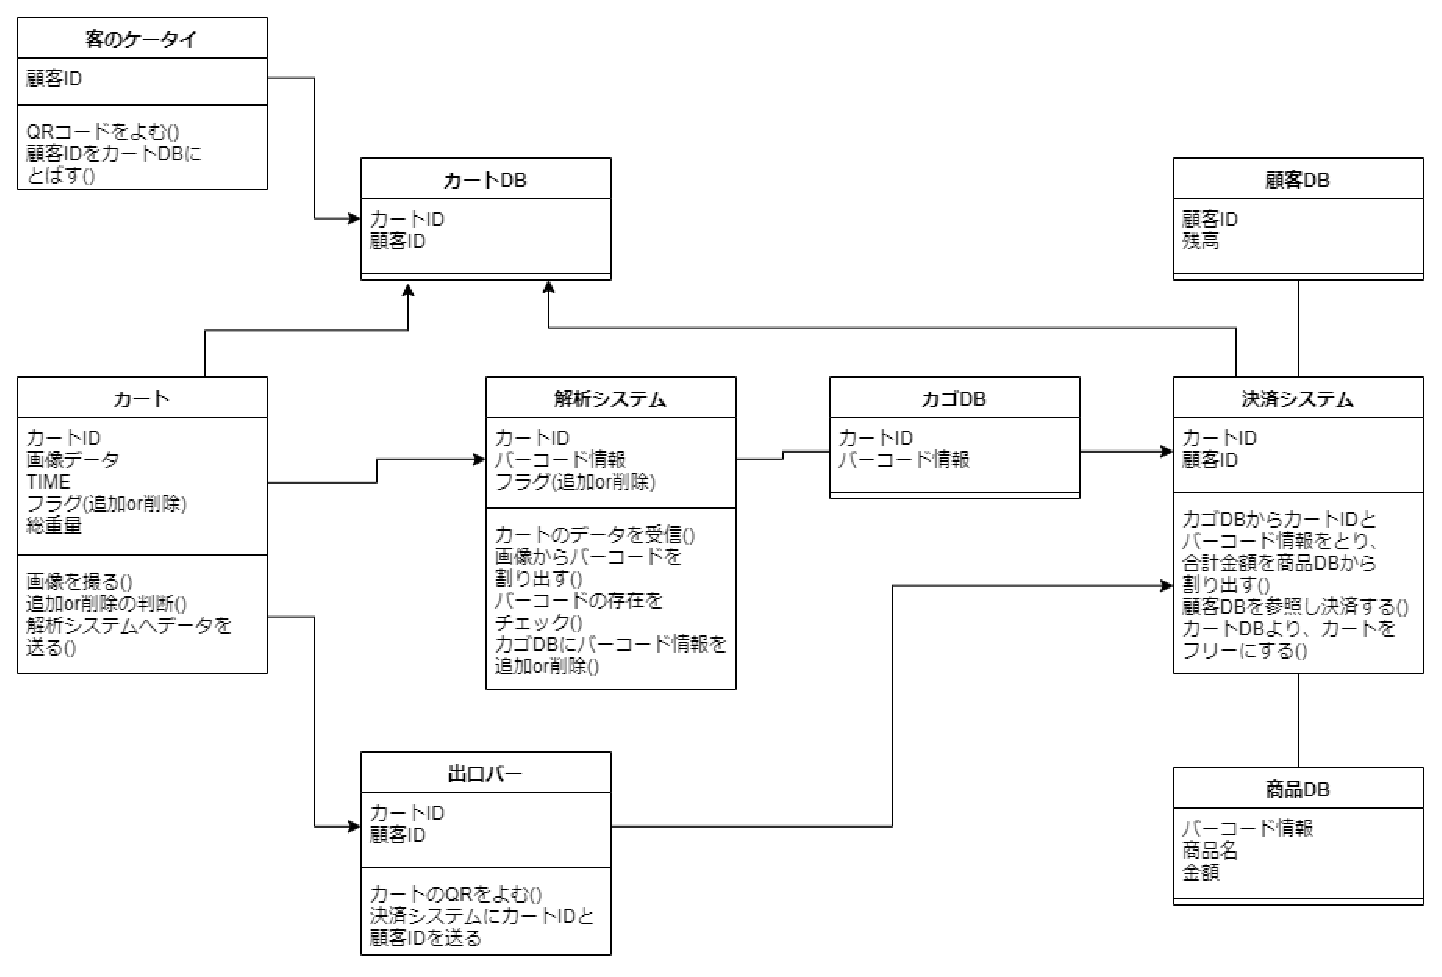
\includegraphics[width=15cm]{./picture/class_qr.eps}
\caption{QRコードを用いたシステムのクラス図}
\label{class_qr}
\end{figure}


本研究では,クラスとしてカート・解析システム・カゴDB・商品DBの部分を開発対象とした.本研究で実装する優先度の高いシステムのクラス図を図\ref{class_qr_2}に示す.


\begin{figure}[htbp]
\centering
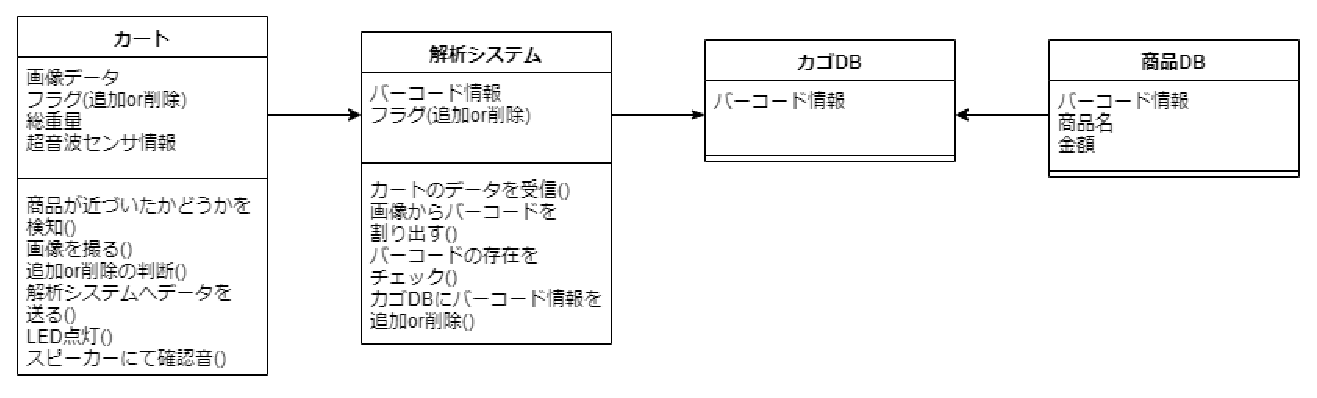
\includegraphics[width=15cm]{./picture/class_qr_2.eps}
\caption{高優先度のシステムのクラス図}
\label{class_qr_2}
\end{figure}